\section{Internationale Arbeitsteilung}
\subsection{Komparativer Kostenvorteil}
\begin{multicols}{2}
	Vorgehen:
	\begin{itemize}
		\item Opportunitätskosten Berechnen für alle Artikel.
		\item Opportunitätskosten vergleichen.
		\item Der Ort mit den tiefsten Opportunitätskosten produziert und
		exportiert zu einem Preis zwischen Opportunitätskosten im
		Exportort und den Opportunitätskosten im Importort (natürlich nur ohne
		Zölle, Transportkosten etc.).
	\end{itemize}
	Falls Gleichstand ist findet kein Handel statt.
	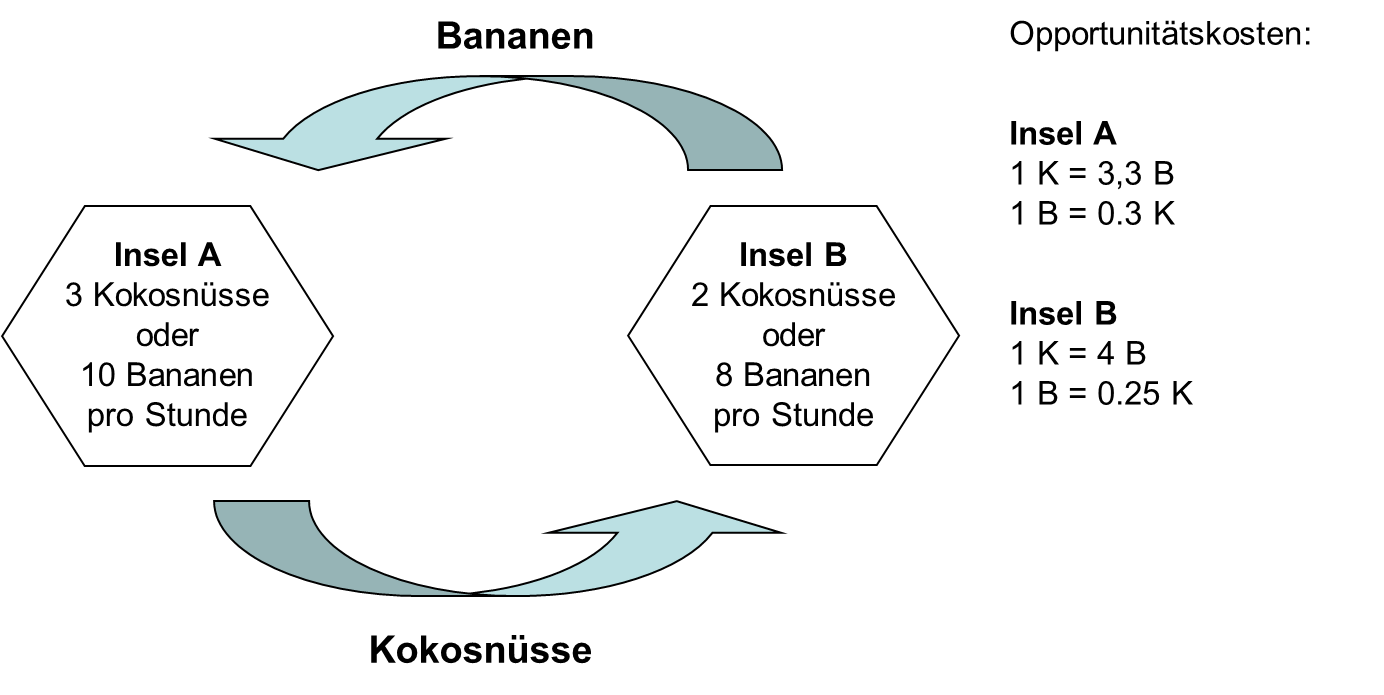
\includegraphics[width=9cm]{images/h03f07.png}
\end{multicols}
\subsection{Weltmarktpreis}
Hoher Weltmarktpreis: Konsument verliert, Allgemeinheit und Produktion gewinnt.\\
Tiefer Weltmarktpreis bewirkt genau das Gegenteil.\\
Internationale Arbeitsteilung bringt positive Wohlfahrtseffekte unabhängig
davon, ob der Weltmarktpreis höher oder tiefer als der Heimmarktpreis ist.
\begin{multicols}{2}
	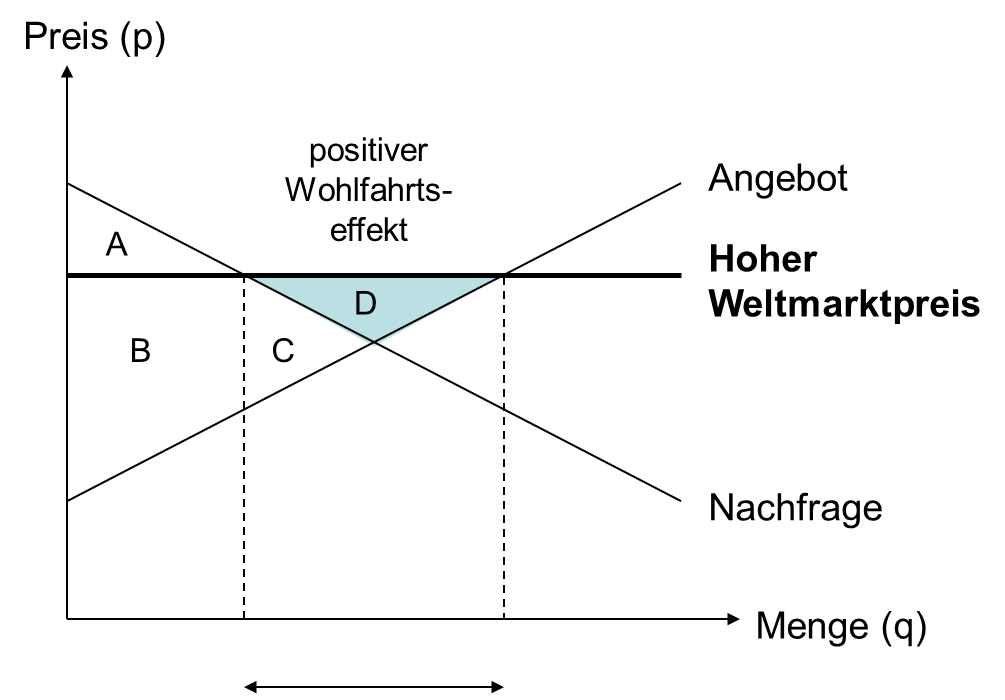
\includegraphics[width=9cm]{images/h03f11.png}\\
	\columnbreak\\
	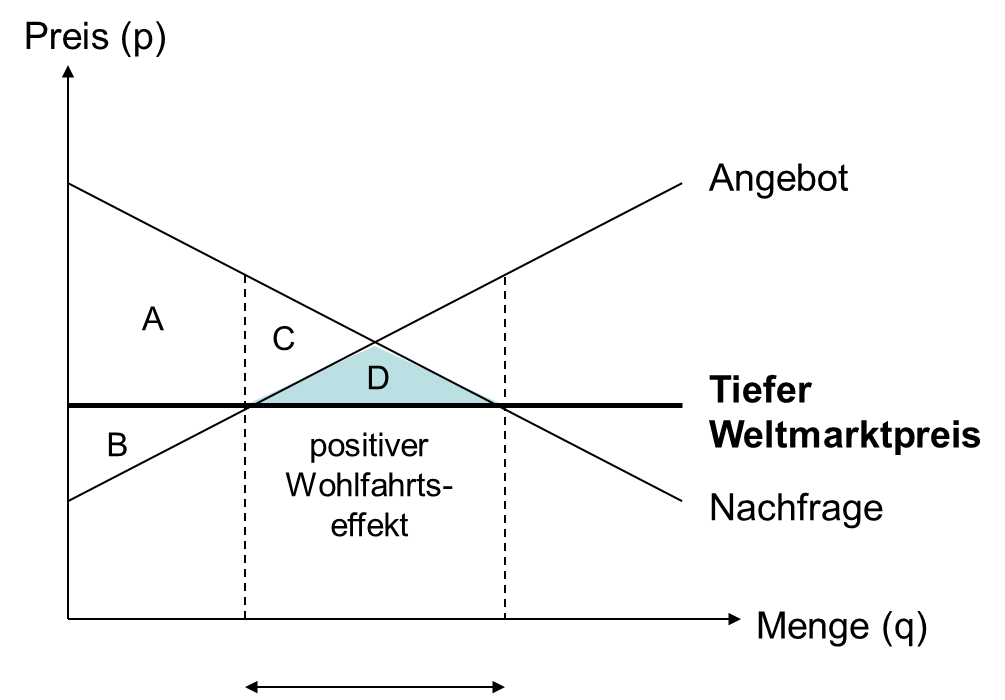
\includegraphics[width=9cm]{images/h03f13.png}
\end{multicols}
\subsection{Protektionismus (Zölle)}
\begin{minipage}{7cm}
	\begin{itemize}
		\item Freihandel bringt eine relativ starke Umverteilung der Wohlfahrt zugunsten des Konsumenten mit sich; dies zu Lasten der Produzenten und des Staates
		\item Der Produzent hat hohes Eigeninteresse, der Konsument nur kleines, daher kann sich oftmals Produzent eher durchsetzten in der Politik
		\item Produzenten sichern sich durch diese Staatseingriffe eine künstliche Rente. Der notwendige Strukturwandel der Wirtschaft wird dadurch verzögert.
	\end{itemize}
\end{minipage}
\begin{minipage}{12cm}
		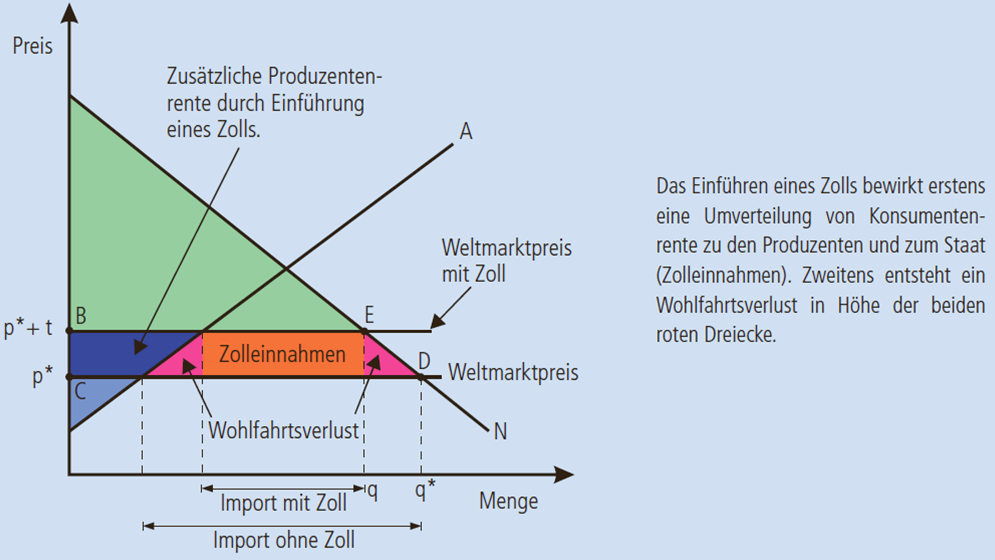
\includegraphics[width=12cm]{images/zolle.png}
\end{minipage}
\subsubsection{Moderne Arten von Zöllen}
\begin{itemize}
	\item Quoten
	\item Technische Handelshemmnisse
	\item Subventionen
	\item Öffentliche Aufträge
\end{itemize}
\subsection{Handelsliberalisierung}
\begin{minipage}{7cm}
	\begin{itemize}
		\item Multilaterale Handelsliberalisierung (WTO)
		\item Regionale Handelsliberalisierung (EU)
		\item Bilaterale Handelsliberalisierung (Der Schweizer-Weg)
	\end{itemize}
	Durch regionale Integration entsteht eine Diskriminierung der Länder, welche nicht Mitglieder des Integrationsraumes sind. Die regionale Integration generiert zusätzlichen Handel, verzerrt diesen aber gleichzeitig. Dadurch entsteht: 
	\begin{itemize}
		\item Handelsschaffung
		\item Handelsumlenkung
	\end{itemize}
\end{minipage}
\begin{minipage}{12cm}
	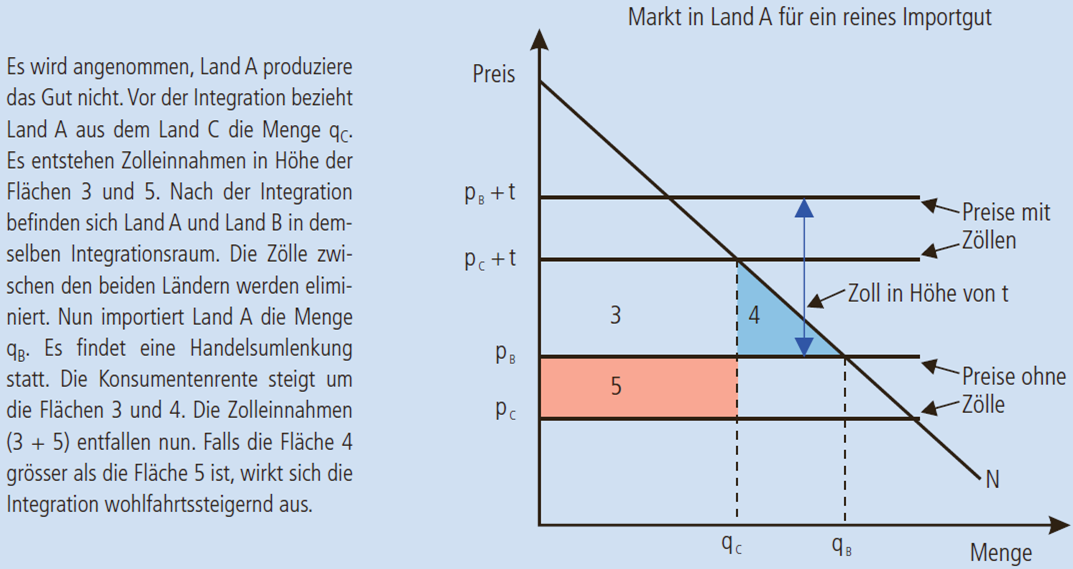
\includegraphics[width=12cm]{images/integrationsraume.png}
\end{minipage}
\subsubsection{Formen von Integrationsräumen}
\begin{figure*}[h]
	\centering
	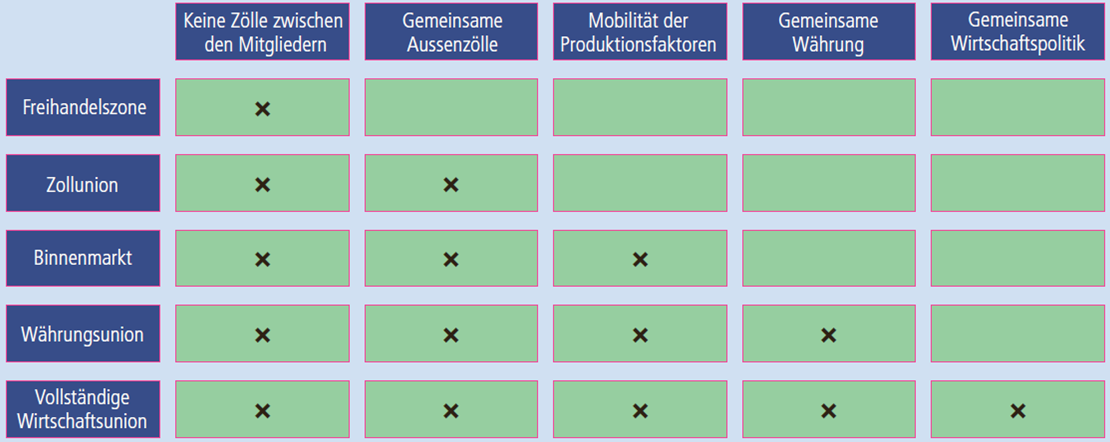
\includegraphics[width=0.75\linewidth]{images/integrationsformen.png}
\end{figure*}